\chapter{Main Conference: Monday, June 23}
\thispagestyle{emptyheader}
\setheaders{Main Conference}{Monday, June 23, 2014}

\clearpage
\setheaders{Parallel Session 1}{\daydateyear}
\begin{ThreeSessionOverview}{Parallel Session 1}{\daydateyear}
  {Semantics (Long Papers)}
  {Tagging, Chunking, Syntax and Parsing (Long + TACL Papers)}
  {Information Retrieval, Text Categorization, Topic Modeling (Long Papers)}
  \marginnote{\rotatebox{90}{11:05}}[2mm]
   \papertableentry{papers-455} & \papertableentry{papers-560} & \papertableentry{papers-533}
\\
 \hline
  \marginnote{\rotatebox{90}{11:30}}[2mm]
   \papertableentry{papers-550} & \papertableentry{papers-136} & \papertableentry{papers-634}
\\
 \hline
  \marginnote{\rotatebox{90}{11:55}}[2mm]
   \papertableentry{papers-670} & \papertableentry{papers-540} & \papertableentry{papers-353}
\\
 \hline
  \marginnote{\rotatebox{90}{12:20}}[2mm]
   \papertableentry{papers-411} & \papertableentry{tacl-488} & \papertableentry{papers-073}
\\
\end{ThreeSessionOverview}

\newpage
\section*{Parallel Session 1}
{\bfseries\large Session 1A: Semantics (Long Papers)}\\
\TrackALoc\hfill\sessionchair{}{}
\paperabstract{\day}{10:40--11:05}{}{}{papers-455}
\paperabstract{\day}{11:05--11:30}{}{}{papers-550}
\paperabstract{\day}{11:30--11:55}{}{}{papers-670}
\paperabstract{\day}{11:55--12:20}{}{}{papers-411}
\clearpage
{\bfseries\large Session 1B: Tagging, Chunking, Syntax and Parsing (Long + TACL Papers)}\\
\TrackBLoc\hfill\sessionchair{}{}
\paperabstract{\day}{10:40--11:05}{}{}{papers-560}
\paperabstract{\day}{11:05--11:30}{}{}{papers-136}
\paperabstract{\day}{11:30--11:55}{}{}{papers-540}
\paperabstract{\day}{11:55--12:20}{}{}{tacl-488}
\clearpage
{\bfseries\large Session 1C: Information Retrieval, Text Categorization, Topic Modeling (Long Papers)}\\
\TrackCLoc\hfill\sessionchair{}{}
\paperabstract{\day}{10:40--11:05}{}{}{papers-533}
\paperabstract{\day}{11:05--11:30}{}{}{papers-634}
\paperabstract{\day}{11:30--11:55}{}{}{papers-353}
\paperabstract{\day}{11:55--12:20}{}{}{papers-073}
\clearpage


\clearpage
\setheaders{Parallel Session 2}{\daydateyear}
\begin{ThreeSessionOverview}{Parallel Session 2}{\daydateyear}
  {Generation and Summarization (Long Papers)}
  {Language and Vision (Long Papers)}
  {NLP for Web, Social Media and Social Sciences (Long Papers)}
  \marginnote{\rotatebox{90}{2:25}}[2mm]
   \papertableentry{papers-055} & \papertableentry{papers-182} & \papertableentry{papers-039}
\\
 \hline
  \marginnote{\rotatebox{90}{2:50}}[2mm]
   \papertableentry{papers-087} & \papertableentry{papers-356} & \papertableentry{papers-524}
\\
 \hline
  \marginnote{\rotatebox{90}{3:15}}[2mm]
   \papertableentry{papers-278} & \papertableentry{papers-420} & \papertableentry{papers-575}
\\
\end{ThreeSessionOverview}

\newpage
\section*{Parallel Session 2}
{\bfseries\large Session 2A: Generation and Summarization (Long Papers)}\\
\TrackALoc\hfill\sessionchair{}{}
\paperabstract{\day}{14:00--14:25}{}{}{papers-055}
\paperabstract{\day}{14:25--14:50}{}{}{papers-087}
\paperabstract{\day}{14:50--15:15}{}{}{papers-278}
\clearpage
{\bfseries\large Session 2B: Language and Vision (Long Papers)}\\
\TrackBLoc\hfill\sessionchair{}{}
\paperabstract{\day}{14:00--14:25}{}{}{papers-182}
\paperabstract{\day}{14:25--14:50}{}{}{papers-356}
\paperabstract{\day}{14:50--15:15}{}{}{papers-420}
\clearpage
{\bfseries\large Session 2C: NLP for Web, Social Media and Social Sciences (Long Papers)}\\
\TrackCLoc\hfill\sessionchair{}{}
\paperabstract{\day}{14:00--14:25}{}{}{papers-039}
\paperabstract{\day}{14:25--14:50}{}{}{papers-524}
\paperabstract{\day}{14:50--15:15}{}{}{papers-575}
\clearpage


\clearpage
\setheaders{Parallel Session 3}{\daydateyear}
\begin{ThreeSessionOverview}{Parallel Session 3}{\daydateyear}
  {Generation and Summarization (Short Papers)}
  {Information Extraction and Question Answering (Short Papers)}
  {Machine Learning for NLP (Short Papers)}
  \marginnote{\rotatebox{90}{3:30}}[2mm]
   \papertableentry{papers-032} & \papertableentry{papers-664} & \papertableentry{papers-227}
\\
 \hline
  \marginnote{\rotatebox{90}{3:45}}[2mm]
   \papertableentry{papers-477} & \papertableentry{papers-446} & \papertableentry{papers-631}
\\
 \hline
  \marginnote{\rotatebox{90}{4:00}}[2mm]
   \papertableentry{papers-570} & \papertableentry{papers-674} & \papertableentry{papers-689}
\\
\end{ThreeSessionOverview}

\newpage
\section*{Parallel Session 3}
{\bfseries\large Session 3A: Generation and Summarization (Short Papers)}\\
\TrackALoc\hfill\sessionchair{}{}
\paperabstract{\day}{15:15--15:30}{}{}{papers-032}
\paperabstract{\day}{15:30--15:45}{}{}{papers-477}
\paperabstract{\day}{15:45--16:00}{}{}{papers-570}
\clearpage
{\bfseries\large Session 3B: Information Extraction and Question Answering (Short Papers)}\\
\TrackBLoc\hfill\sessionchair{}{}
\paperabstract{\day}{15:15--15:30}{}{}{papers-664}
\paperabstract{\day}{15:30--15:45}{}{}{papers-446}
\paperabstract{\day}{15:45--16:00}{}{}{papers-674}
\clearpage
{\bfseries\large Session 3C: Machine Learning for NLP (Short Papers)}\\
\TrackCLoc\hfill\sessionchair{}{}
\paperabstract{\day}{15:15--15:30}{}{}{papers-227}
\paperabstract{\day}{15:30--15:45}{}{}{papers-631}
\paperabstract{\day}{15:45--16:00}{}{}{papers-689}
\clearpage


{\section{SRW Poster Session}
{\setheaders{SRW Poster Session}{\daydateyear}
6:00--9:00\\
\posterabstract{srw-004}
\posterabstract{srw-007}
\posterabstract{srw-011}
\posterabstract{srw-012}
\posterabstract{srw-013}
\posterabstract{srw-017}
\posterabstract{srw-023}
\posterabstract{srw-024}
\posterabstract{srw-028}
\posterabstract{srw-029}
\posterabstract{srw-030}
\posterabstract{srw-031}
\posterabstract{srw-040}
\posterabstract{srw-043}
\posterabstract{srw-047}
\posterabstract{srw-049}
\posterabstract{srw-051}
\posterabstract{srw-053}
\posterabstract{srw-056}
\posterabstract{srw-058}
\posterabstract{srw-059}
\posterabstract{srw-060}
\posterabstract{srw-062}


{\section{Poster session 1A}
{\setheaders{Poster session 1A}{\daydateyear}
6:00--7:30\\
\posterabstract{papers-069}
\posterabstract{papers-123}
\posterabstract{papers-125}
\posterabstract{papers-167}
\posterabstract{papers-169}
\posterabstract{papers-205}
\posterabstract{papers-229}
\posterabstract{papers-232}
\posterabstract{papers-243}
\posterabstract{papers-263}
\posterabstract{papers-315}
\posterabstract{papers-367}
\posterabstract{papers-379}
\posterabstract{papers-421}
\posterabstract{papers-497}
\posterabstract{papers-521}
\posterabstract{papers-525}
\posterabstract{papers-529}
\posterabstract{papers-531}
\posterabstract{papers-541}
\posterabstract{papers-557}
\posterabstract{papers-589}
\posterabstract{papers-591}
\posterabstract{papers-595}
\posterabstract{papers-605}
\posterabstract{papers-617}
\posterabstract{papers-697}
\posterabstract{papers-699}
\posterabstract{papers-701}
\posterabstract{tacl-255}
\posterabstract{tacl-371}
\posterabstract{tacl-381}
\posterabstract{tacl-385}
\posterabstract{tacl-403}
\posterabstract{tacl-429}
\posterabstract{tacl-485}


{\section{Poster session 1B}
{\setheaders{Poster session 1B}{\daydateyear}
7:30--9:00\\
\posterabstract{papers-056}
\posterabstract{papers-090}
\posterabstract{papers-116}
\posterabstract{papers-150}
\posterabstract{papers-172}
\posterabstract{papers-178}
\posterabstract{papers-196}
\posterabstract{papers-218}
\posterabstract{papers-222}
\posterabstract{papers-226}
\posterabstract{papers-274}
\posterabstract{papers-296}
\posterabstract{papers-298}
\posterabstract{papers-306}
\posterabstract{papers-322}
\posterabstract{papers-336}
\posterabstract{papers-404}
\posterabstract{papers-428}
\posterabstract{papers-438}
\posterabstract{papers-448}
\posterabstract{papers-460}
\posterabstract{papers-552}
\posterabstract{papers-578}
\posterabstract{papers-586}
\posterabstract{papers-590}
\posterabstract{papers-648}
\posterabstract{tacl-452}
\posterabstract{tacl-472}


\newpage
%% % Cut-and-pasted from auto/papers/Monday.tex, then manually hand-edited

\section*{Overview}
\renewcommand{\arraystretch}{1.2}
\begin{SingleTrackSchedule}
  7:30 & -- & 6:00 &
  {\bfseries Registration} \hfill (\RegistrationLoc)
  \\
  7:30 & -- & 9:00 &
  {\bfseries Breakfast} \hfill (\BreakfastLoc)
  \\
  8:55 & -- & 9:00 &
  {\bfseries Opening session} \hfill (\PlenaryLoc)
  \\
  9:00 & -- & 9:40 &
  {\bfseries Presidential Address: Gertjan van Noord} \hfill (\PlenaryLoc)\index{van Noord, Gertjan}
  \\
  9:40 & -- & 10:10 &
  {\bfseries Coffee break} \hfill (\BreakLoc)
  \\
  10:10 & -- & 11:50 &
  \begin{tabular}{|p{.65in}|p{.65in}|p{.65in}|p{.65in}|p{.65in}|}
    \multicolumn{5}{l}{{\bfseries Session 1}}\\\hline
  \small (\TrackALoc) & \small (\TrackBLoc) & \small (\TrackCLoc) & \small (\TrackDLoc) & \small (\TrackELoc) \\\hline
Discourse, Dialogue, Coreference and Pragmatics & Semantics I & Machine Translation I & Syntax, Parsing, and Tagging I & NLP for the Web and Social Media I \\
  \hline\end{tabular} \\
  11:50 & -- & 1:20 &
  {\bfseries Lunch break; Bloomberg and Nuance Student Lunch} \hfill (\StudentLunchLoc)
  \\
  1:20 & -- & 3:00 &
  \begin{tabular}{|p{.65in}|p{.65in}|p{.65in}|p{.65in}|p{.65in}|}
    \multicolumn{5}{l}{{\bfseries Session 2}}\\\hline
Syntax, Parsing and Tagging II & Semantics II & Word Segmentation and POS Tagging & SRW Thesis Proposal Presentations & Sentiment Analysis I \\
  \hline\end{tabular} \\
  3:00 & -- & 3:30 &
  {\bfseries Coffee break} \hfill (\BreakLoc)
  \\
  3:30 & -- & 4:45 &
  \begin{tabular}{|p{.65in}|p{.65in}|p{.65in}|p{.65in}|p{.65in}|}
    \multicolumn{5}{l}{{\bfseries Session 3}}\\\hline
Topic Modeling & Information Extraction I & Generation & Syntax, Parsing and Tagging III & Language Resources and Evaluation I \\
  \hline\end{tabular} \\
  4:45 & -- & 5:00 &
  {\bfseries Break} \hfill (\BreakLoc)
  \\
  5:00 & -- & 6:00 &
  {\bfseries Keynote address: Corinna Cortes} \hfill (\PlenaryLoc)
  \\
  6:05 & -- & 6:50 &
  {\bfseries Student Research Workshop Oral Highlights} \hfill (\SRWLoc)
  \\
  6:50 & -- & 9:30 &
  {\bfseries Poster and Dinner Session I: TACL Papers, Long Papers, Short Papers, Student Research Workshop, Demonstrations} \hfill (\PosterSessionLoc)
  \\
\end{SingleTrackSchedule}
\newpage
%% \input{content/day2/monday-schedule}\newpage
%% \input{content/day2/monday-schedule}\newpage
%\thispagestyle{myheadings}
\section{Keynote Address: Corinna Cortes}
\index{Cortes, Corinna}

\begin{center}

\begin{Large}
{\bfseries\Large ``Learning Ensembles of Structured Prediction Rules''}\vspace{1em}\par
\end{Large}

%% \begin{center}
%%   \begin{tabular}{m{1in}b{1in}}
%%     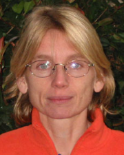
\includegraphics[width=1in]{content/monday/cortes-headshot.png}
%%     & {\bfseries Corinna Cortes} \newline Google Research, NY
%%   \end{tabular}
%% \end{center}

\daydateyear, 5:00--6:00pm \vspace{1em}\\
\PlenaryLoc \\
\vspace{1em}\par
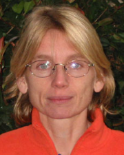
\includegraphics[height=100px]{content/monday/cortes-headshot.png}
\end{center}

\noindent
{\bfseries Abstract:} We present a series of algorithms with
theoretical guarantees for learning accurate ensembles of several
structured prediction rules for which no prior knowledge is assumed.
This includes a number of randomized and deterministic algorithms
devised by converting on-line learning algorithms to batch ones, and a
boosting-style algorithm applicable in the context of structured
prediction with a large number of labels. We also report the results
of extensive experiments with these algorithms.

This is joint work with Vitaly Kuznetsov, NYU, and Mehryar Mohri, NYU/Google
Research.

\vspace{3em}\par 

\vfill
\noindent

{\bfseries Biography:} Corinna Cortes is the Head of Google Research,
NY, where she is working on a broad range of theoretical and applied
large-scale machine learning problems. Prior to Google, Corinna spent
more than ten years at AT\&T Labs - Research, formerly AT\&T Bell Labs,
where she held a distinguished research position. Corinna's research
work is well-known in particular for her contributions to the
theoretical foundations of support vector machines (SVMs), for which
she jointly with Vladimir Vapnik received the 2008 Paris Kanellakis
Theory and Practice Award, and her work on data-mining in very large
data sets for which she was awarded the AT\&T Science and Technology
Medal in the year 2000. Corinna received her MS degree in Physics from
University of Copenhagen and joined AT\&T Bell Labs as a researcher in
1989. She received her Ph.D. in computer science from the University
of Rochester in 1993. Corinna is also a competitive runner.

\newpage
\newpage

%\section{Oral Presentations}
%\vspace{1em}\par\centerline{\bfseries\Large Paper Abstracts}\vspace{1em}\par
\addcontentsline{toc}{section}{Parallel Sessions}
%% \input{auto/main/monday-main-abstracts.tex}
\newpage

% I'm bypassing the \section command here because I didn't like the layout
% from the ACL-IJNLP handbook that I started from. UG

%% \setheaders{NAACL HLT: Poster and Demonstrations Session}{Monday, June 10, 2013}

%% \section{Poster Madness!}

%% Prior to the poster session, poster presenters are given one minute each to pitch their
%% paper. Posters from the Student Research Workshop are included. Following the Poster Madness!
%% session, there will be a buffet dinner and a combined Posters and Demonstrations session.

%% \noindent
%% \vspace{1em}\par\centerline{\bfseries\large Main Conference Posters}\vspace{1em}\par
%% \input{auto/main/main-poster-abstracts.tex}

%% \noindent
%% \vspace{1em}\par\centerline{\bfseries\large Student Research Workshop Posters}\vspace{1em}\par
%% \noindent
%% %% \input{auto/srw/monday-srw-1.tex}
%% \input{auto/srw/monday-srw-1-B-abstracts.tex}

%% \clearpage
%% \section{Posters and Demonstrations Session}

%% The Poster and Demonstrations Session will be held in the Grand Atrium of the 200 Building from
%% 6:30--8:30pm, and will include a buffet dinner. The Demonstrations abstracts are printed below,
%% since they were not a part of the Poster Madness! session.

%% \noindent
%% %% \input{auto/demo/monday-demo-1.tex}
%% \input{auto/demo/demo-poster-abstracts.tex}
